\documentclass[12pt,a4paper,UTF8]{ctexart}
\usepackage{amsmath}
\usepackage{graphicx}
\usepackage{float}
\usepackage{listings}
\usepackage{xcolor}
\usepackage{geometry}
\usepackage{booktabs}
\usepackage{hyperref}

\geometry{left=2.5cm,right=2.5cm,top=2.5cm,bottom=2.5cm}

% 代码样式设置
\lstset{
    language=Python,
    basicstyle=\ttfamily\small,
    keywordstyle=\color{blue},
    commentstyle=\color{gray},
    stringstyle=\color{red},
    numbers=left,
    numberstyle=\tiny\color{gray},
    stepnumber=1,
    numbersep=8pt,
    backgroundcolor=\color{gray!10},
    frame=single,
    breaklines=true,
    captionpos=b
}

\title{HW1实验报告\\CIFAR-10图像分类与动量优化对比}
\author{刘继轩 \\ 学号:2400017722}
\date{\today}

\begin{document}

\maketitle

\section{实验概述}
本实验主要包含两个部分:
\begin{enumerate}
    \item \textbf{Part 1} 使用PyTorch框架构建卷积神经网络(CNN)对CIFAR-10数据集进行图像分类训练。
    \item \textbf{Part 2} 对比在SGD优化器中不同动量(momentum)参数值对模型训练效果的影响。
\end{enumerate}

\section{数据集介绍}
CIFAR-10是一个经典的图像分类数据集,包含10个类别的彩色图像:
\begin{itemize}
    \item 类别:飞机(plane)、汽车(car)、鸟(bird)、猫(cat)、鹿(deer)、狗(dog)、青蛙(frog)、马(horse)、船(ship)、卡车(truck)
    \item 图像尺寸:32×32像素,3通道RGB彩色图像
    \item 训练集:50,000张图像
    \item 测试集:10,000张图像
\end{itemize}

\section{模型架构}
\subsection{网络结构}
本实验采用了经典的LeNet变体架构,具体结构如下:

\begin{table}[H]
\centering
\caption{cifarNet网络结构}
\begin{tabular}{@{}lll@{}}
\toprule
层类型 & 参数配置 & 输出尺寸 \\
\midrule
输入 & - & 3×32×32 \\
卷积层1 & 3→6, kernel=5×5 & 6×28×28 \\
最大池化1 & kernel=2×2, stride=2 & 6×14×14 \\
卷积层2 & 6→16, kernel=5×5 & 16×10×10 \\
最大池化2 & kernel=2×2, stride=2 & 16×5×5 \\
展平层 & - & 400 \\
全连接层1 & 400→120 & 120 \\
全连接层2 & 120→84 & 84 \\
全连接层3 & 84→10 & 10 \\
\bottomrule
\end{tabular}
\end{table}

\subsection{数据预处理}

使用torchvision中的datasets下载cifar-10数据集,并利用transforms对输入图像进行了以下预处理:
\begin{enumerate}
    \item 转换为张量格式(ToTensor)。
    \item 像素值归一化(Normalize):使用均值0.5和标准差0.5进行归一化,将像素值范围从[0,1]映射到[-1,1]。
\end{enumerate}

\subsection{超参数设置}
\begin{itemize}
    \item 学习率(learning rate):0.001
    \item 批量大小(batch size):8
    \item 训练轮数(epochs):10
    \item 优化器:SGD,动量(momentum)参数在实验中进行调整。
\end{itemize}

\subsection{其他设计细节}
\begin{itemize}
    \item 所有隐藏层(卷积层和全连接层)使用ReLU激活函数。
    \item 使用交叉熵损失函数(CrossEntropyLoss)作为多分类任务的损失函数。
    \item 使用随机梯度下降(SGD)作为优化器。
\end{itemize}

\section{\textbf{Part 1} 基础实验结果}

在Part 1中,我们使用`momentum=0.9`进行训练。训练10个epoch后,模型在测试集上的整体准确率为62.51\%。各类别的准确率如下:

\begin{figure}[H]
    \centering
    % 左:表格,右:图片,并排放置,强制顶端对齐
    \begin{minipage}[t]{0.3\textwidth}
        \centering
        \vspace{0pt} % 强制顶端对齐
        \small
        \begin{tabular}{@{}lc@{}}
        \toprule
        类别 & 准确率(\%) \\
        \midrule
        plane & 56.20 \\
        car & 81.00 \\
        bird & 54.60 \\
        cat & 42.50 \\
        deer & 66.30 \\
        dog & 35.50 \\
        frog & 69.30 \\
        horse & 69.50 \\
        ship & 77.10 \\
        truck & 73.10 \\
        \bottomrule
        \end{tabular}
        \caption{各类别准确率}
        \label{tab:class_accuracy}
    \end{minipage}
    \hfill
    \begin{minipage}[t]{0.6\textwidth}
        \centering
        \vspace{0pt} % 强制顶端对齐
        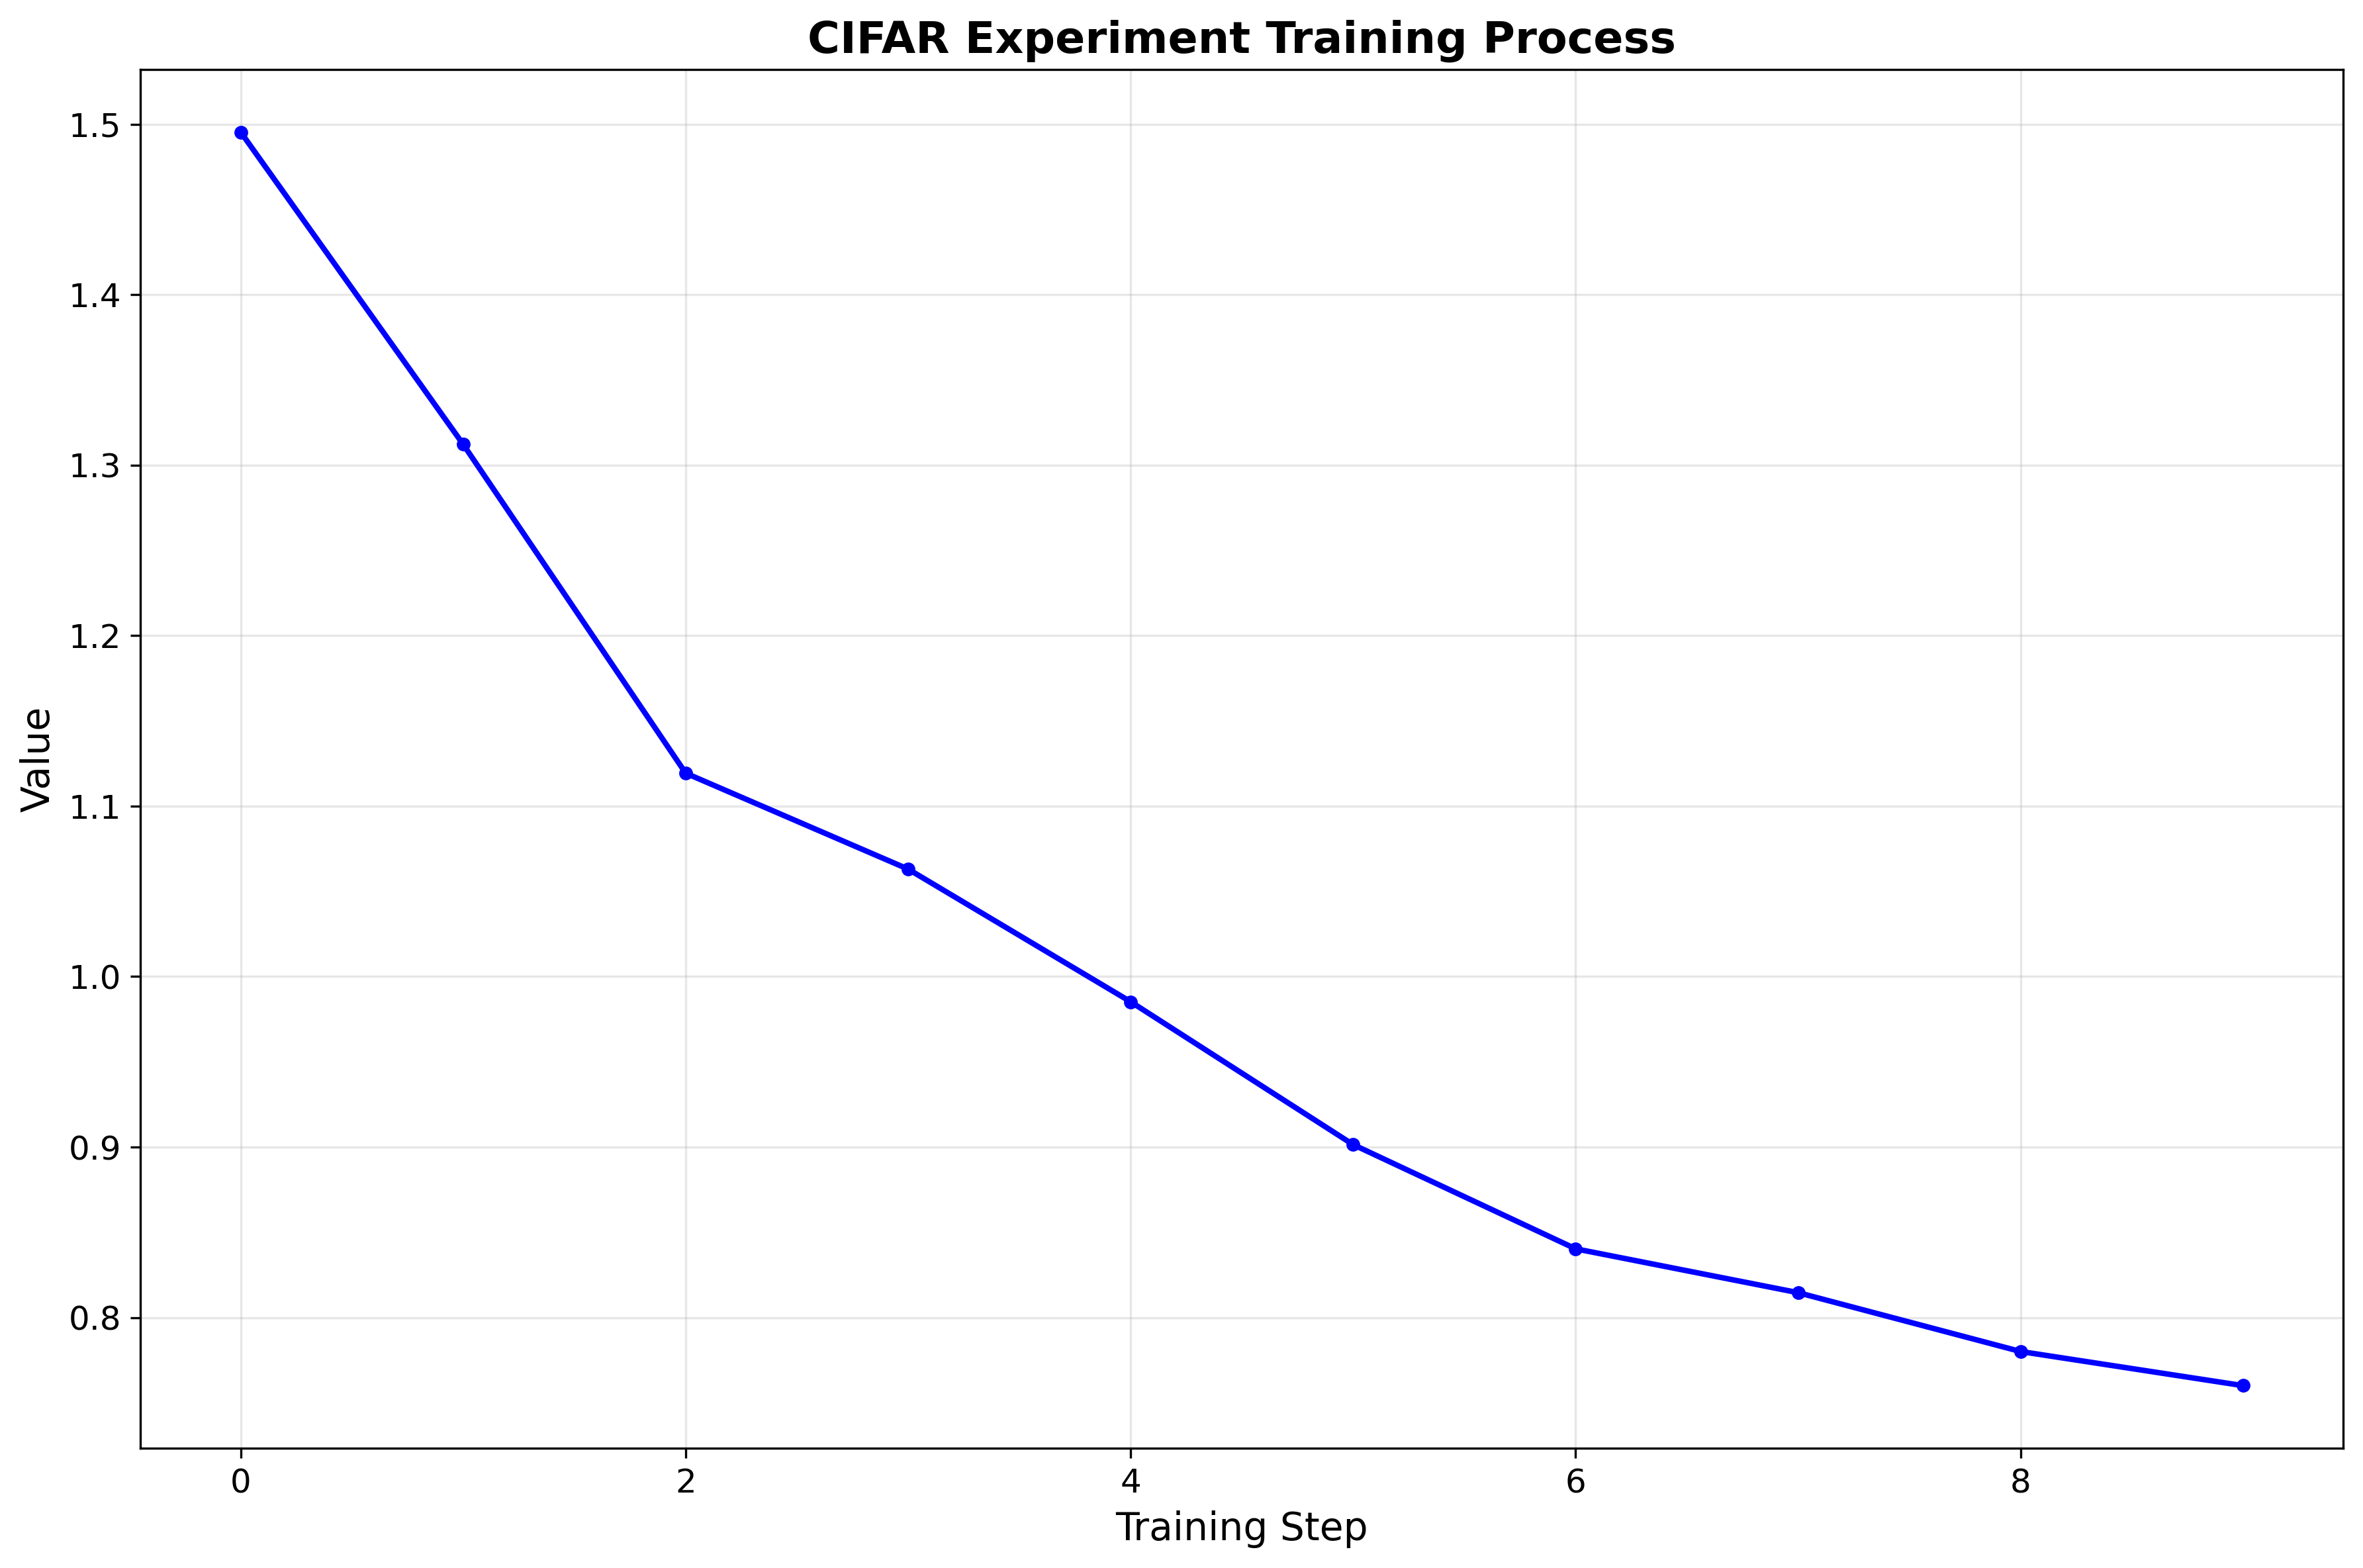
\includegraphics[width=\linewidth]{./cifar_experiment_plot.png}
        \caption{训练损失曲线 (momentum=0.9)}
        \label{fig:loss_curve}
    \end{minipage}
\end{figure}

从结果可以看出,模型已能有效拟合训练数据,损失函数稳步下降。然而,模型在“猫”和“狗”等类别上表现较差,这可能是由于这些类别内部差异较大,且当前模型结构简单,未采用数据增强、正则化等高级技巧,导致泛化能力有限。

\section{\textbf{Part 2} 动量参数对比实验}

动量(momentum)是SGD优化器中的一个重要超参数,它通过积累历史梯度信息来加速收敛并减少优化过程中的振荡。

\subsection{实验设计}
为研究动量参数对训练效果的影响,我们设计了对照实验。在固定随机数种子以保证实验可复现的前提下,我们测试了四种不同的动量值,并观察其训练损失曲线和最终测试准确率:
\begin{itemize}
    \item momentum = 0.0 (无动量)
    \item momentum = 0.5 (中等动量)
    \item momentum = 0.9 (较高动量,常用值)
    \item momentum = 0.99 (极高动量)
\end{itemize}

\subsection{动量对比实验结果}
图\ref{fig:momentum_comparison}展示了不同动量值下的损失函数收敛曲线。

\begin{figure}[H]
    \centering
    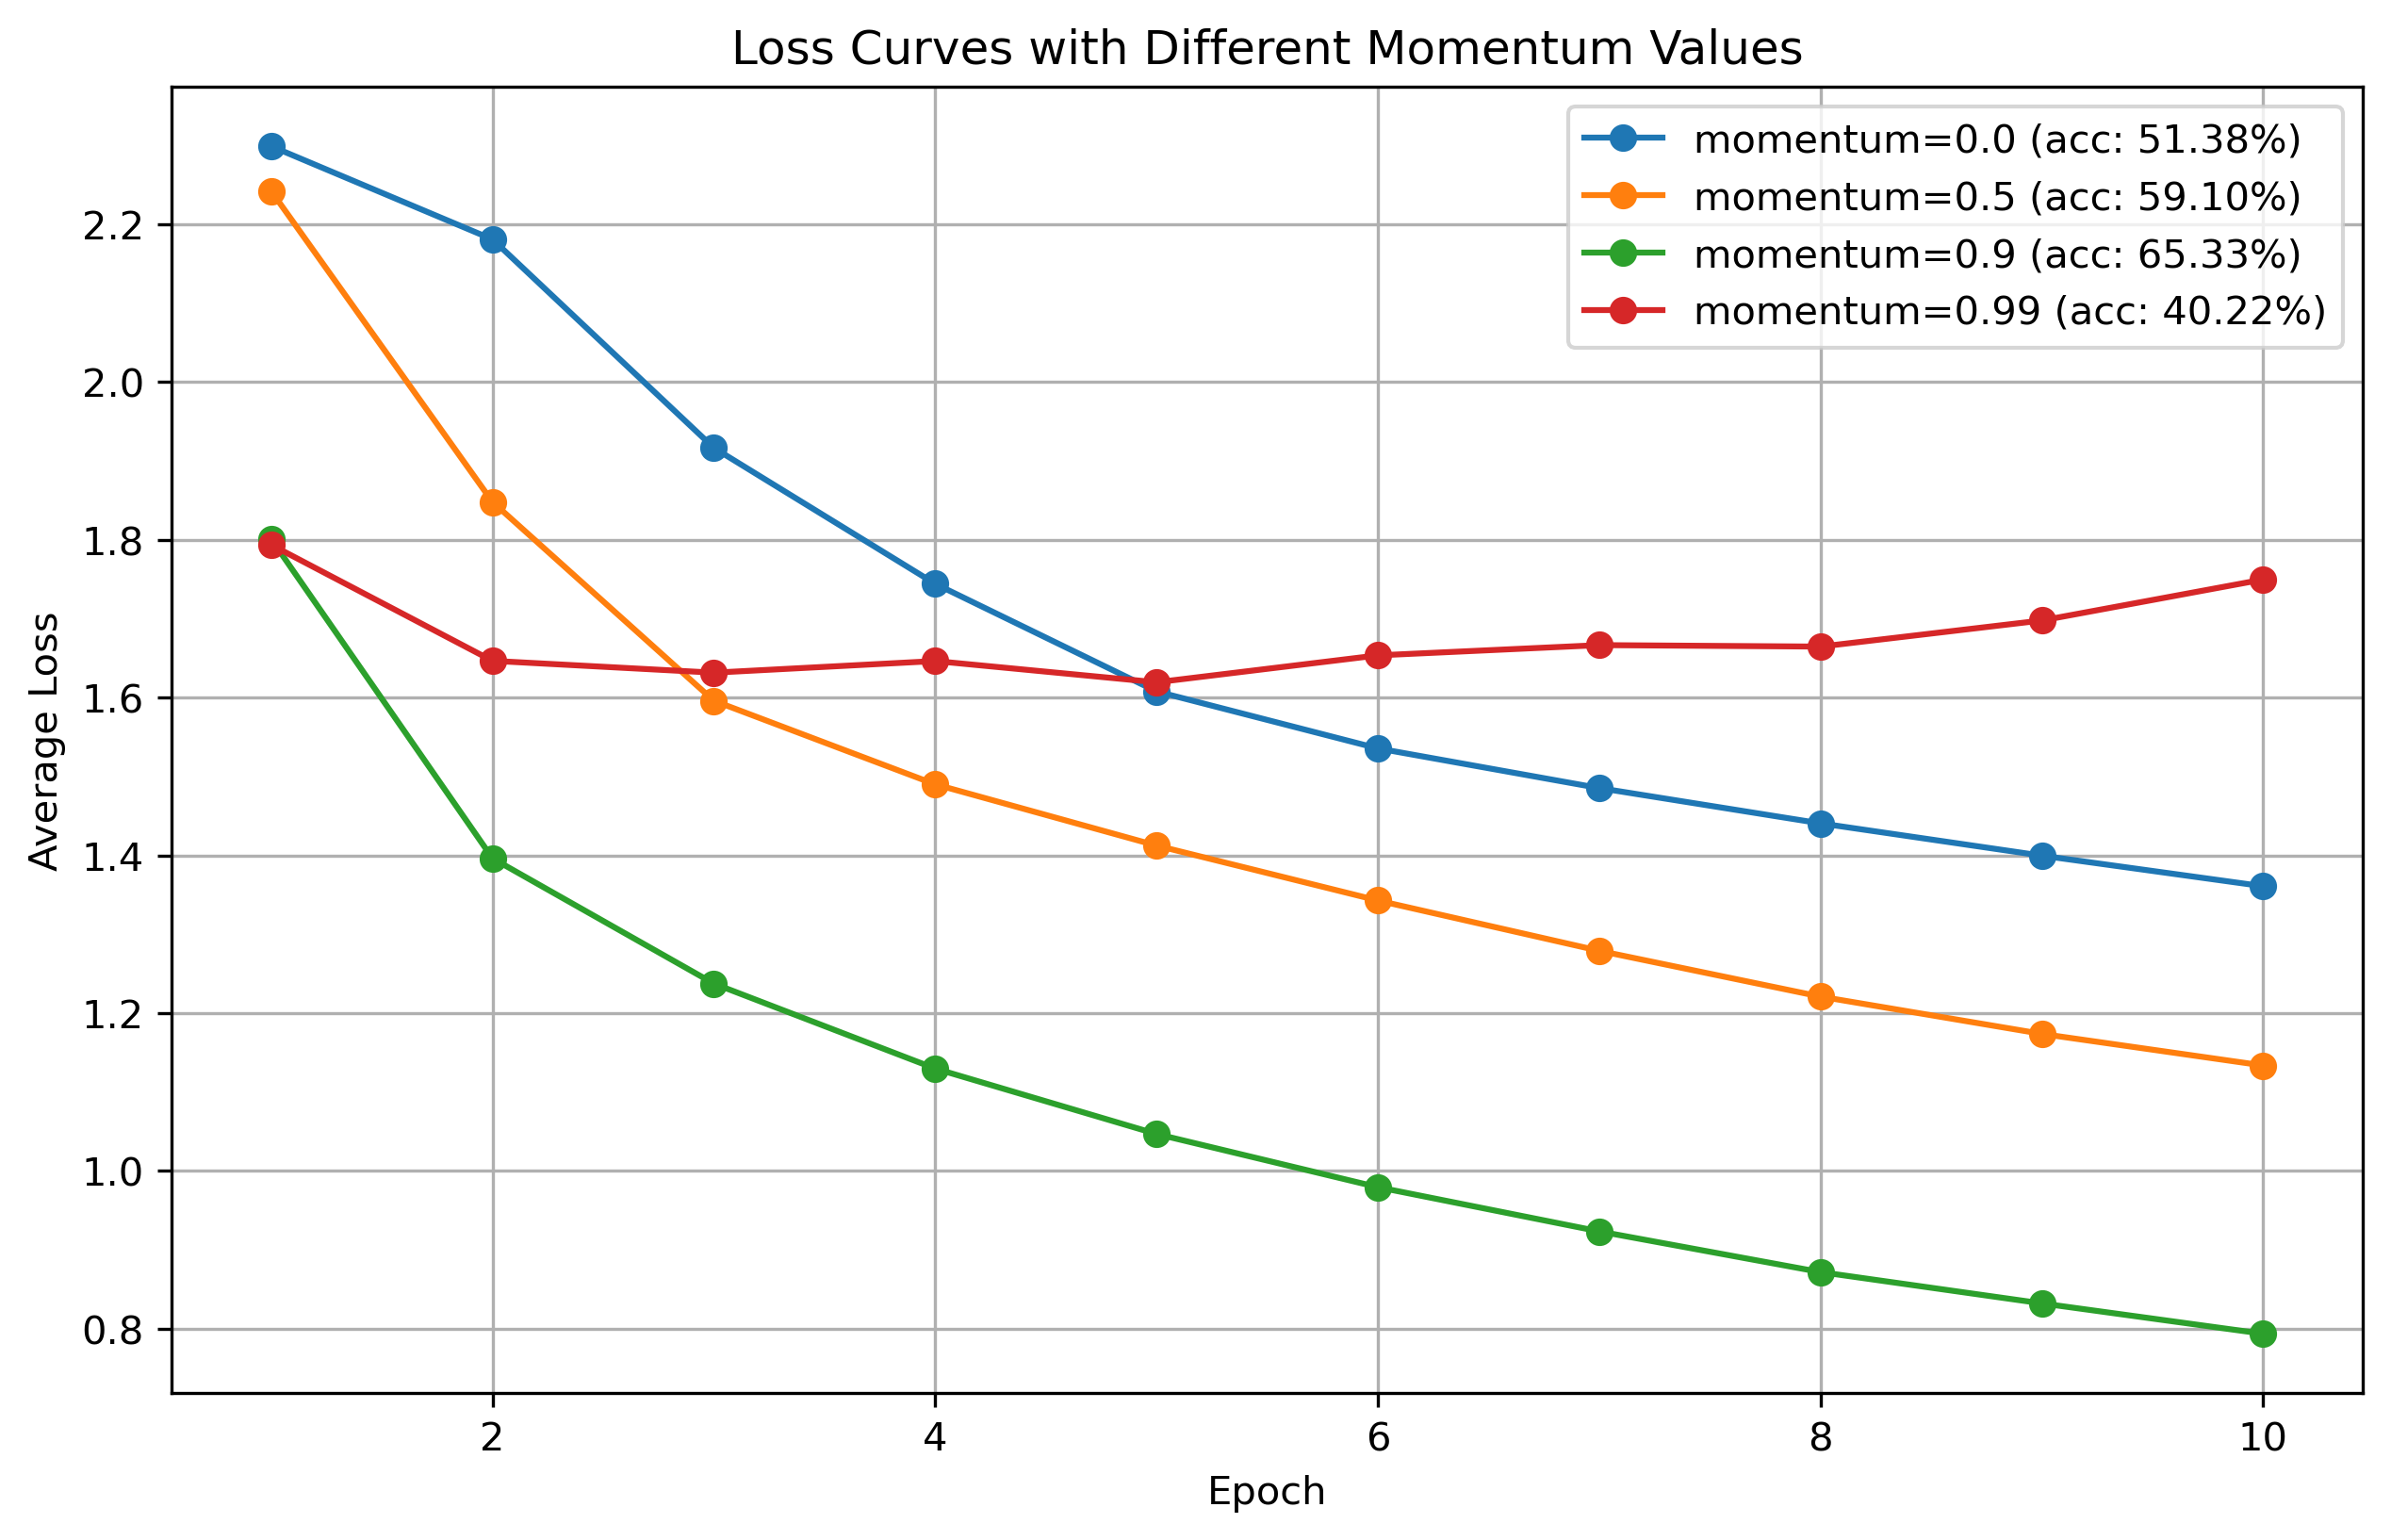
\includegraphics[width=0.8\textwidth]{momentum_comparison.png}
    \caption{不同动量值的损失函数对比}
    \label{fig:momentum_comparison}
\end{figure}

各动量值对应的最终测试准确率如表\ref{tab:momentum_accuracy}所示。

\begin{table}[H]
\centering
\caption{不同动量值的测试准确率对比}
\begin{tabular}{@{}cc@{}}
\toprule
动量值 & 测试准确率(\%) \\
\midrule
0.0 & 51.38 \\
0.5 & 59.10 \\
0.9 & 65.33 \\
0.99 & 40.22 \\
\bottomrule
\end{tabular}
\label{tab:momentum_accuracy}
\end{table}

\section{结果分析与讨论}
\subsection{动量对训练的影响}
从实验结果可以观察到以下几个重要现象:

\begin{enumerate}
    \item \textbf{适中动量效果最佳}:`momentum=0.9`时获得了最高的测试精度(65.33\%),表现最好。
    \item \textbf{无动量收敛较慢}:`momentum=0.0`时,损失函数下降最为缓慢,最终精度也相对较低(51.38\%)。
    \item \textbf{过高动量可能有害}:`momentum=0.99`时,虽然早期损失下降最快,但很快出现剧烈振荡,最终精度反而最低(40.22\%)。这可能是因为过大的动量导致更新步长过大,使得优化器“冲过”了最优点,并在其附近来回震荡,难以收敛到更精细的局部最小值。
    \item \textbf{收敛稳定性}:`momentum=0.5`和`0.9`都展现出了良好的收敛稳定性,损失函数持续下降。
\end{enumerate}

\subsection{理论解释}
动量机制在SGD中的工作原理可以简化为以下公式:
\begin{equation}
v_t = \beta v_{t-1} + \nabla_\theta J(\theta_t)
\end{equation}
\begin{equation}
\theta_{t+1} = \theta_t - \alpha v_t
\end{equation}

其中,$\beta$是动量系数(momentum),$\alpha$是学习率,$v_t$是当前时刻的动量(梯度的指数移动平均),$\nabla_\theta J(\theta_t)$是当前参数的梯度。

\begin{itemize}
    \item \textbf{动量的优势}:当梯度方向连续保持一致时,动量项会累积,从而加速收敛;当梯度方向变化时,动量项可以抵消部分振荡,使优化路径更平滑。
    \item \textbf{过高动量的问题}:过大的$\beta$值意味着历史梯度的影响过重,可能导致更新步长太大而“冲过”最优点(overshooting),使其难以在最优解附近稳定下来。
    \item \textbf{最优选择}:通常0.9被认为是一个在多种任务中表现稳健的默认值,本实验的结果也支持了这一经验。
\end{itemize}

\section{实验总结}
\subsection{主要收获}
\begin{enumerate}
    \item 成功实现了基于CNN的CIFAR-10图像分类任务,在简单模型下达到了65.33\%的测试精度。
    \item 通过对比实验,深入理解了动量参数对深度学习模型训练速度和最终性能的重要影响。
    \item 掌握了PyTorch框架的核心使用流程,包括数据加载、模型定义、训练循环和模型评估。
    \item 学会了使用TensorBoard对训练过程(如损失曲线)进行可视化,为模型调试和分析提供了有力工具。
\end{enumerate}

\end{document}